%   MSc Business Analytics Dissertation
%
%   Title:     Literature Review
%   Author: Conor Reid
%
%   Chapter 3: Literature Review
%
\chapter{Literature Review}\label{C.LitReview}
\section{Introduction}\label{S.intro3}
{This literature review first presents some of the ways that corporate success can be quantified. This includes how it is defined by \cite{moldovan2015learning}, as well as by others whose approaches may benefit this study. This is followed by an analysis of literature pertaining to the relationship between corporate governance and company performance, again including the work of \cite{moldovan2015learning} as well as other relevant studies. This review finishes with an exploration of literature regarding causation and the statistical techniques used to infer causation. There is also discussion on the issues that arise in attempting to do so, and how they can be addressed. }
\section{Company Performance - Measures and Factors}
{Among the key aspects of this study is the quantifying of corporate success, in a way that accurately   represents good and bad corporate performance. There are many aspects to this. For example, many different financial ratios have been developed that attempted to assign numerical performance ratings to companies taking into account a variety of accounting indictors. \cite {eidleman1995z} states that these ratios are often created by academics, and outlined the patterns they tend follow. He desribes how researchers find a sample of companies that meet some predetermined criterion of failure, as well as another sample of comparable firms (size, industry etc) that differ only in financial health. Common statistical learning can then be used to analyse which ratios can accurately separate the groups. Those which do so are kept, the rest discarded. Weights are assigned to each ratio to reach an aggregate equation. New firms are scored, and real-world performance recorded to measure how useful the new ratios are. \\\\
Blindly following financial ratios is often suboptimal and can be thought of as an over-reliance on simple stock price indicators. Perhaps the inclusion of more varied and diverse measures are required, such as the companies social responsibility commitments, and their impact on the environment. Both may contribute to a more accurate picture of corporate performance, and are discussed below.       }
\subsection{Financial Ratios}
{One of the indicators of corporate performance used by \cite{moldovan2015learning} is Tobin's Q score. This measure was devised by \cite{tobin1969general} who postulated that the combined market value of a given company should be equal to their replacement costs. This is described as the ideal state, with any deviation either way (a ratio above or below 1) warranting investment or the selling of assets. The use of this measure is well established in the literature, by \cite{chung1994simple}, 
\cite{bhagat2008corporate} and \cite{bolton2011unified}. \cite{chung1994simple} state that Tobin's Q plays an important part in financial interactions, and is employed to explain diverse corporate phenomena during the decision making process. \cite{bolton2011unified} used Tobin's Q to propose a model for dynamic investment and risk management and found that investment is best driven by the Q score as well as to the marginal value of liquidity.\\\\
The formal definition of Tobin's Q is given by \cite{chung1994simple} as; 
\begin {equation}\label{TobinQ}
L-R  \quad q = \small {\frac{PREFST + VCOMS + LTDEBT + STDEBT - ADJ}{TOTASST - BKCAP + NETCAP}}
\end{equation}\\
There is debate as to the practically of the Q score. \cite{chung1994simple} go on to state that the Q score is often neglected in real-world situations. One of the reasons they give for this is the complexity of the necessary calculations, and a potential unfamiliarity with its operational intricacies. Another reason is the unavailability of relevant data, particularly with high accuracy and in real-time. To counteract this, they worked to create and test an accurate approximation of Tobin's Q that utilises only basic financial information. They conclude that their approximation is close enough to the more formal definition to be used where more exhaustive calculations are not possible. \\\\
\cite {dybvig2010tobin} criticise Tobin's Q more strongly, stating that it is fundamentally malformed as a measure of corporate performance. They highlight long-serving managers as risk adverse, and who "...can {\it enjoy the quiet life} and underinvest". A logical implication of this is that firms invest less and operate well below their profit-generating capacity and thus reduces their net-present value. However, such is Tobin's Q formulated, underinvestment by a firm increases its Q score. They go on to explain the scores ambiguity, COME BACK TO. \\\\Another measure of corporate success used by \cite{moldovan2015learning} is the Altman Z score, which is often used as a probabilistic measure of whether a company will go into bankruptcy within the next two years. It can also be used more generally as a financial distress measure and to predict corporate defaults. The authors point out that there is much advocacy in the literature for using this measure, and this study was unable to find any that strongly reject its usefulness. The Altman Z score is given as;
\begin {equation}\label{AltmanZScore}
\begin{aligned}
Z \ Score \quad = \quad & 1.2\bigg(\frac{Working \ Capital}{Total \ Assets}\bigg) \ + \\\\
		& 1.4\bigg({\frac{Retained \ Earnings}{Total \ Assets}}\bigg) \ + \\\\
		& 3.3\bigg({\frac{Earnings \ before \ Interest \ and \ Tax}{Total \ Assets}}\bigg) \ + \\\\
		& 0.6\bigg({\frac{Market \ Value \ of \ Equity}{Total \ Liabilities}}\bigg) \ + \\\\
		& 1.0\bigg({\frac{Sales}{Total \ Assets}}\bigg)
\end{aligned}
\end{equation}\\
Among those that support this scores use is \cite {eidleman1995z}, who discusses its use in practice. He begins by highlighting Altman's own tests using the Z score which involved predicting 72\% of bankruptcies two years prior to the event, although the sample size or companies involved are not mentioned. Eidleman argues that the Z score is tried and tested, and;
\begin {quote}
It has been demonstrated to be quite reliable in a variety of contexts and countries. 

\hspace{2cm}---  \cite {eidleman1995z}
\end{quote}
Eidleman also outlines circumstances that warrant corrections and alterations to equation \ref{AltmanZScore}, in order to generalise it beyond its originally intended means. He argues that before being able to use the Z score, one must ensure the company in question is comparable to those involved in Altman's original study. Altman considered manufacturing and small firms in his original analysis, thus corrections must be made before scoring companies in different industries. Eidelman points to two specific circumstances here. \\\\
The first considers privately held companies, whose stocks are no publicly traded meaning term four of equation \ref{AltmanZScore} cannot be calculated. To correct for this, the Z score can be re-estimated using book values of equity. In other words, details from balance sheets published by private firms voluntarily can be used rather than details gleamed from the stock market. Certainly a work-around here is to consider solely publicly traded companies. A consequence of this is that such an analysis would only include companies that are bound by the the corporate governance code in their jurisdiction, which would need to be taken into account in studies such as this one.\\\\ Eidleman's second consideration is for non-manufacturing firms. The fifth term of equation \ref{AltmanZScore}, according to Eidleman, varies significantly by industry. He argues that merchandise firms for example, are significantly less capital intense and thus are much more likely to enjoy higher asset turnover and consequently Z-Scores. Z scores then would be likely to under-predict bankruptcy in these cases. In order to correct for this, a recommendation comes from Altman to eliminate the fifth term and adjust the weights. The adjusted equation \ref{AltmanZScoreAjusted} is shown below;
\begin {equation}\label{AltmanZScoreAjusted}
\begin{aligned}
Z \ Score \quad =  \quad & 6.56\bigg(\frac{Working \ Capital}{Total \ Assets}\bigg) \ + \\\\
		& 3.26\bigg({\frac{Retained \ Earnings}{Total \ Assets}}\bigg) \ + \\\\
		& 6.72\bigg({\frac{Earnings \ before \ Interest \ and \ Tax}{Total \ Assets}}\bigg) \ + \\\\
		& 1.05\bigg({\frac{Market \ Value \ of \ Equity}{Total \ Liabilities}}\bigg) \ \\\\ 
\end{aligned}
\end{equation}\\
Overall, the Altman Z score seems a highly appropriate indicator of corporate financial strength and thus success, and one that should be considered in this study. Consideration will need to be had for the type of industry included in this analysis, that will inform the exact calculation of the Z score itself. }
\subsection{Environmental Considerations}
{As mentioned previously, there is likely much room for improvement in quantifying corporate success beyond financial ratios. One potentially useful alternative is the link between environmental and economic performance, studied by \cite{schaltegger2002link}. If it is possible to draw relationships between these two areas, environmental considerations may be introduced into the model to good effect. The authors present two conflicting viewpoints in this space. The first states that improved environmental performance predominantly causes an increase in operating costs, which in turn negatively effects the profitability of the company. The second viewpoint states the opposite; improving a firms environmental performance in fact induces cost savings, which drives increases in profitability. These viewpoints are visualised in figure \ref{ch3_successAndEnviornment}. 
\begin{figure}[h] 
\centering
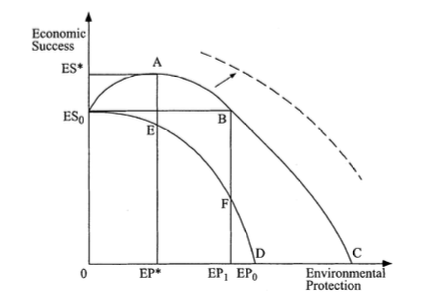
\includegraphics[scale = 0.7]{images/ch3_successAndEnviornment.png}
\caption{Potential correlations between corporate environmental protection and economic success.}
\label{ch3_successAndEnviornment}
\end{figure}\\
$ES_0$ represents the current level of economic success (this is described as a certain shareholder value), which decreases as spending in environmental protection increases (through points E and F, to D where non profit can be made). This is the pessimistic view, or the expectation that spending in this space reduces profit making ability to eventual zero. The more optimistic view is represented by the path from $ES_0$ through points A and B to point C (again where no profit is possible). This represents the ideology that some economic gain can be achieved, at least to some degree before tailing off, by investing in the environmental space. \\\\
The authors research discusses both viewpoints and offers a framework for their coexistence. Ultimately, they argue it is the method with which a firm achieves a certain level of environmental performance that best correlates with economic success, rather than a simple binary indicator for whether they undertook to do so or not. They reframe the question, saying;
\begin{quote}
The question whether it pays to be green is insufficient and that rather the question which should be investigated is when it pays to be green.

\hspace{2cm}--- \cite{schaltegger2002link}
\end{quote}
It follows that not every kind of environmental management increases economic success, a conclusion that informs the authors framework for best managing efforts to increase environmental performance in right way. \\\\
It is clear that environmental success can be a good indicator for economic success, and may prove useful to include in this study as independent variables that have potential predict power for corporate success. 
}
\subsection{Corporate Responsibility}
\section{Corporate Governance and Company Performance}
\subsection{Governance Models}
\subsection{Measures of Company Performance}
\subsection{Influence of Governance on Performance}
\section{Inferring Causation}
\subsection{Introduction}
\subsection{Techniques}
\subsection{Examples}